\section{Clustering comparison}
	
	In this section a series of clustering algorithm are compared
	
	\subsection{The data}
	
		There are 4 different types of datasets:
		\begin{itemize}
			\item Zernike coefficients
			\item PSF
			\item LP coefficients
			\item Photonic Lantern Output fluxes
		\end{itemize}
		
		The paths to the datasets can be found in the file \href{https://github.com/Dacarpe03/PLImageReconstruction/blob/main/Utils/minidataset_constants.py}{minidataset\_constants.py}.\\
		
		We have used 2, 5, 9, 14 and 20 zernike modes to create 5 datasets of 5000 datapoints each.
		
	\subsection{Results}
		\begin{figure*}[ht!]
			\centering
			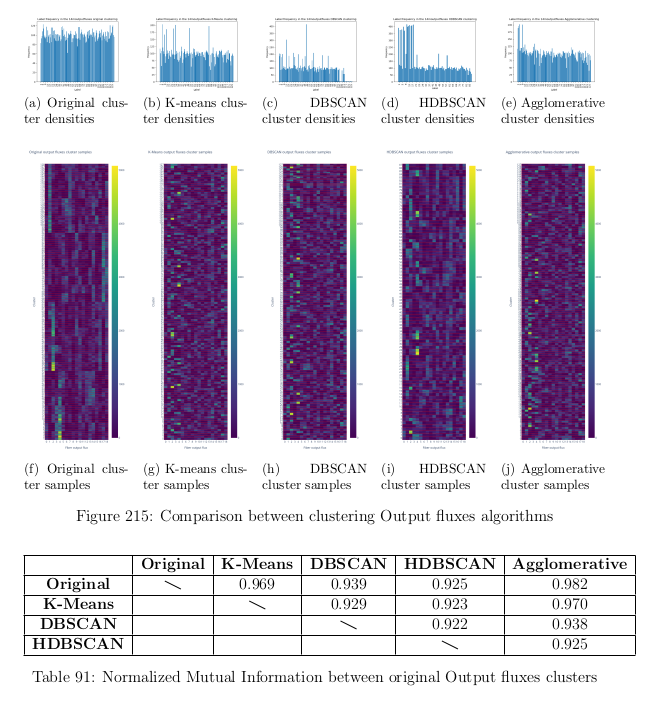
\includegraphics[width=0.9\textwidth]{
		draft-20clustersummary.png}
			\caption{Summary of clustering 20 zernike modes dataset}
		\end{figure*}
		\FloatBarrier
		
		The best clustering algorithm is the Agglomerative followed by K-Means, although K-Means takes a lot of time.
		
	\subsection{Detailed results}
	
		For a detailed report on the datasets, results and plots see Part IV to VII from \filename{all.pdf}.